\documentclass{../source/Experiment}

\major{信息工程}
\name{姚桂涛}
\title{基于GNURadio的FM发送与接收}
\expname{基于GNURadio的FM发送与接收}
\stuid{3190105597}
\college{信息与电子工程学院}
\date{\today}
\lab{东4-319}
\course{通信原理实验}
\instructor{金向东、龚淑君}
\grades{}
\exptype{验证性实验}
\partner{叶慷鹏}
\begin{document}
\section{实验目的和要求}

    在 GNURadio Companion 软件平台下,基于 USRP B210 硬件设备搭建搭建 FM 发射机发送音频信号并搭建 FM 收音机收听 FM 广播

    \section{实验电路分析}


    \begin{figure}[H]
        \centering
        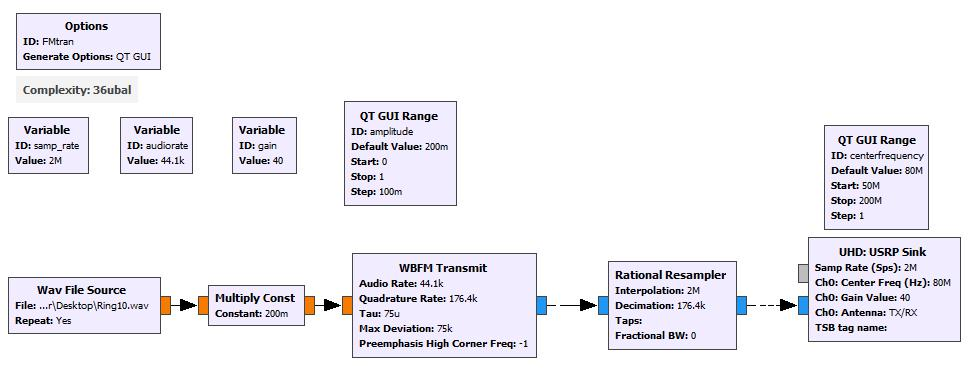
\includegraphics[width = 0.8\textwidth]{lab7-2}
        \caption{FM发射信号流图}
    \end{figure}
    
    \begin{figure}[H]
        \centering
        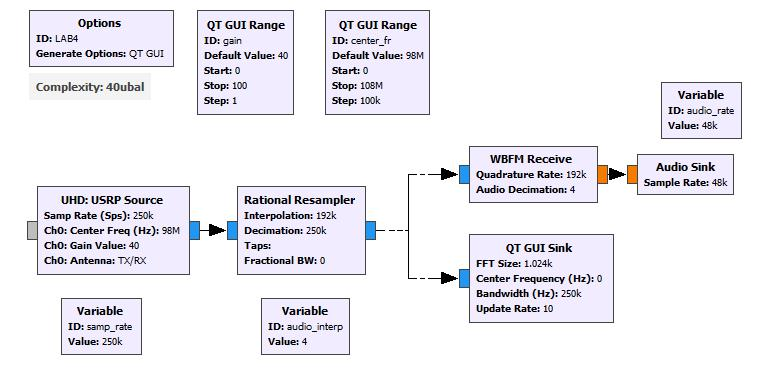
\includegraphics[width = 0.8\textwidth]{lab7-1}
        \caption{FM接收信号流图}
    \end{figure}


    \section{实验数据与结果分析}
        \subsection{幅度调制实验}
            \subsubsection{普通幅度调制(AM)}
            JP3端由高频信号源输入频率为465kHz,大小为0dBm的正弦波作为载波信号输入;JP2端
            由信号源输入频率为1kHz,大小为0dBm的正弦波作为调制信号;接通跳线J3的1、2端或者2、
            3端;将平衡调节电位器WR1逆时针或顺时针旋到底。
            
            此次实验我们采用时域法调制度测量。

            用示波器观察调制输出信号波形(注意,示波器观察时将频谱分析仪的电缆从JP4脱开,
            避免信号被衰减):双通道观测,以JP2端输入的调制信号为示波器的触发源,观察调制输出
            TP4波形,测量其调制度。改变调制信号幅度,或调节平衡调节电位器WR1,分别将调制度调
            整到30\%、50\%和100\%,记录相应波形。
            
            \subsubsection{双边带调制(DSB)}

            在普通幅度调制的基础上,调节电位器WR1,同时观察信号频谱,直到频谱中载波分量降到最低,这就实现抑制载波幅度调制(DSB)。用示波器观察并记录调制输出信号的波形(注意,将频谱分析仪的电缆从JP4脱开)。

        \subsection{同步相干解调实验}

        \subsubsection{AM 同步解调}

        调整WR1,使调制电路产生AM调制信号,用示波器观测同步解调输出信号。改变JP2端调制信号幅度,从而改变已调波信号的调制度,观察同步解调输出信号的幅度变化。

        \subsubsection{DSB 同步解调}
        
        调整WR1,使调制电路产生DSB调制信号,用示波器观测同步解调输出信号。改变JP2端调制信号幅度,观察同步解调输出信号的幅度变化。

        \subsection{包络检波实验}
        
        \subsubsection{包络检波信号的测量}
        
        由高频信号源从JP4端输入载波频率为465kHz,大小为10dBm(即2Vp-p),调制信号频率为1kHz的正弦波,调制度为30\%的AM调幅信号。

        (1) 改变跳线 J1,选择不同的时间常数,用示波器在测试点 TP8观察检波输出信号的惰性失真情况。

        (2) 改变跳线 J2,选择不同的交流阻抗,用示波器在测试点 TP10观察检波输出信号的负峰切割失真情况。

        (3) 在无失真的情况下,改变输入信号的调制度,观察对输出信号的影响(何时出现失真)?

    \section{思考题}
	    \subsection{AM、DSB 调制有何区别,它们分别是如何实现的}
        
        \subsection{已调波信号的调制度与什么因素有关系?}

        \subsection{包络检波输出信号产生惰性失真和负峰切割失真的原因分别是什么?如何改善失真情况?}
        
        \subsection{DSB 调制信号是否可以通过包络检波方式进行解调?
        }
	
\end{document}